\section{Aero-elastic galloping}
\numberwithin{figure}{section}
In this section the behavior of a flexible, elastic structure, when it is subject to heavy wind. These structures can produce or sustain large amplitude oscillations, as will be evidenced by the analytical and numerical results. In this section an infinitesimal element a bridge is considered. This infinitesimal is portrayed in figure \ref{fig:ex2galloping}.
\begin{figure}[htp]
\centering
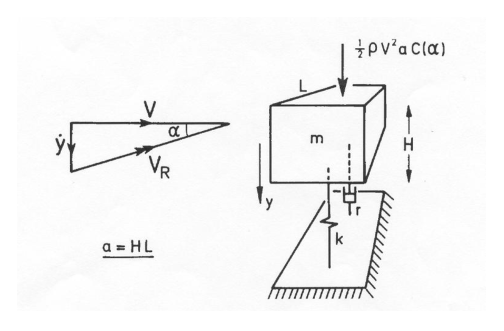
\includegraphics{img/ex2/galloping.eps}
\caption{}
\label{fig:ex2galloping}
\end{figure}

The forces that act on this element in the vertical direction are
\begin{itemize}
\item \textit{Inertia: $m\cdot \ddot{y}$}
\item \textit{Linear damping: $r\cdot\dot{y}$}
\item \textit{Elastic force: $k\cdot{y}$}
\item \textit{Driving force:} The wind relative to the prism $V_R$ is also shown in figure \ref{fig:ex2galloping}. Since the wind $V$ is purely horizontal, the vertical force due to $V_R$ will be a function of $\dot{y}$. For small $\alpha$ or equivalently large $V$, the angle $\alpha$ can be approximated by $\alpha=\frac{\dot{y}}{V}$ ($\sin{\theta}\approx \theta$ for small $\theta$). The force along the direction of the speed $\dot{y}$ is then given by
\begin{equation}
\frac{1}{2}\cdot\rho V^2aC(\alpha)
\end{equation}
where $C(\alpha)$ can be approximated by the 7th order polynomial
\begin{equation}\label{eqn:ex2calpha}
C(\alpha) = A_1\cdot \alpha-A_3 \cdot \alpha^3 + A_5\cdot \alpha^5 - A_7\cdot \alpha^7
\end{equation}
Met $\alpha$ expressed in radials, and the coefficiants $A_i$ as given in the assignment. This driving force can be seen as a nonlinear damping due to it being a function of $\dot{y}$
\end{itemize}
The full equations of the prism's motion are then given by
\begin{equation}\label{eqn:ex2model1line}
m\ddot{y}=-r\dot{y}-ky+\frac{1}{2}\rho V^2 a A_1 C(\alpha)
\end{equation}
\hfill\newline
Note that while the elastic force and the linear damping will counteract the accelaration, the driving force will increase it. When considering the system from now on the following values will be used
 \begin{equation}\label{eqn:ex2numericvalues}
m=1,\rho=1,r=1,k=100,a=1
\end{equation}

\subsection{A linear approximation}
First, the second order model equation (\ref{eqn:ex2model1line}) must be reduced to two first order equations
 \begin{align}
 \frac{dy}{dt}&=\dot{y}\label{eqn:dydt}\\
 \frac{d\dot{y}}{dt}&=-\frac{r}{m}\dot{y}-\frac{k}{m}y+\frac{1}{2m}\rho V^2 a A_1 C(\alpha)\label{eqn:ddotydt}
 \end{align}
 To find fixed points, $\frac{dy}{dt}$ as well as $\frac{d\dot{y}}{dt}$ must be zero. From the first condition it is found that $\dot{y}$ must be zero. This condition in (\ref{eqn:ddotydt}) then leads to $y=0$. So the origin is the only possible fixed point. In order to investigate it's stability, the system must be linearised. The only nonlinear term is the one containing $C(\alpha)$, which when linearising and evaluating in $0$ leads to $A_1$. The linearised system is then given by
 \begin{equation}
\begin{bmatrix}\frac{dy}{dt}\\\frac{d\dot{y}}{dt}\end{bmatrix}=\begin{bmatrix}0 & 1\\ -k & -r+\frac{1}{2}\rho VaA_1\end{bmatrix}\begin{bmatrix}y \\ \dot{y}\end{bmatrix}
\end{equation}
When using the values of \ref{eqn:ex2numericvalues} the Jacobian matrix and its trace and determinant become
\begin{equation}
J=\begin{bmatrix}0 & 1 \\-100 & -1+\frac{1}{2}VA_1\end{bmatrix}, \tau=-1+\frac{1}{2}VA_1, \Delta=100
\end{equation}
\hfill\newline
Since $\Delta$ is always positive, the fixed point will be a stable or unstable spiral  when $\tau<\sqrt{4\Delta}=20$. It's stability depends on $\tau$. When $V=V_C=\frac{2}{A_1}$, a bifurcation occurs when the real parts of the complex eigenvalues switch sign. When $V>V_C$, $\tau>0$ and the spiral is unstable. When $V<V_C$, $\tau<0$ and the spiral is stable. When only considering this linear model, the bifurcation that occurs is a degenerate Hopf bifurcation. When $V=V_C$ there will be a continuous band of closed orbits surrounding the origin.
\subsection{Simulating the system}
The system can be simulated using a SIMULINK model, shown in figure \ref{fig:ex1simmodel}. With this model the value of $V/V_c$ can be adapted during the simulation. The interpretations from the linearised model are checked with the full equations. When $V<V_C$, the fixed point is indeed stable. When increasing $V$ above $V_C$ however, a limit cycle appears. The fixed point at the origin is indeed an unstable spiral, but the appearance of the limit cycle points to a supercritical Hopf bifurcation instead of a degenerate Hopf bifurcation. This limit cycle can be explained when looking at (\ref{eqn:ex2calpha}), in the case $\alpha<1$. When $V>Vc$, this means that the coefficient of $\dot{y}$ in the driving force is greater then coefficient of $\dot{y}$ in the Linear damping when only considering the term $A_1\cdot \alpha$. This then leads to unstable behavior in every point of the $(y,\dot{y})$ plane. However, when also taking into account the term $-A_3\cdot \alpha^3$, the behavior will be stable for large values of $\alpha$ because the Driving force is weaker than the Linear damping. Thus, points very far from the origin are attracted towards it, and points near the origin are repelled from it. This explains the observed limit cycle.
\begin{figure}[htp]
\centering
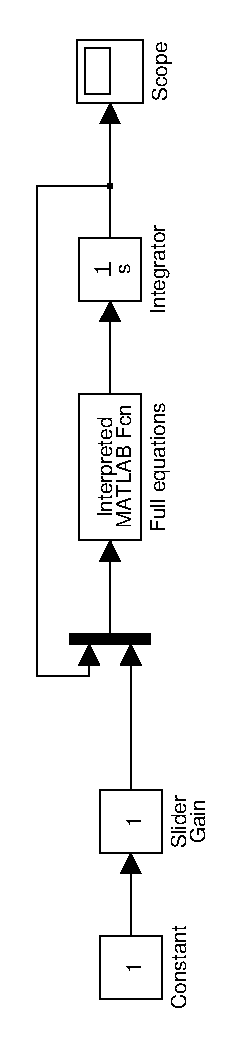
\includegraphics[angle=-90,trim= 0mm 7mm 5mm 10mm]{img/ex1/model1.eps}
\caption{}
\label{fig:ex1simmodel}
\end{figure}
\newline
When during the simulations $V$ is further increased, the radius of the limit cycle will suddenly jump to a distant value. When afterwards decreasing the $V$ again, the radius decreases continuously from the distant value, until it jumps again to a lower value. These two jumps are saddle-node bifurcations of cycles, as a stable and an unstable cycle collide and annihilate. Figure \ref{fig:ex227b} shows the evolution of the radius of the limit cycle for increasing $V$ on a step-by-step basis. The initial condition goes to zero, and when $V/V_C$ is increased, the two jumps in the amplitudes of the limit cycles become visible. Figure \ref{fig:ex227} at the end of this section shows a qualitative study in the $(y,\dot{y})$-space. In each subplot, the value of $V/V_C$ is increased by 0.2. The starting point of the simulation is denoted by a red dot. The simulation is carried out until a stable orbit is reached, which is shown in green. When $V/V_C$ is increased above 1, the first stable limit cycle appears. For increasing $V/V_C$, the radius of this limit cycle becomes wider and wider (Note that the axes are scaled so as to make the orbits appear circular).  When $V/V_C$ is increased above 1.8 to 2, the radius suddenly jumps to a distant value. When again decreasing $V/V_C$, the orbits steadily decrease from this value, until jumping back to the first stable limit cycle when $V/V_C$ is lowered below 1.4.  
\begin{figure}[htp]
\centering

\includegraphics{img/ex2/27b.eps}
\caption{}
\label{fig:ex227b}
\end{figure}

\subsection{Bifurcation diagrams}
From the previous section, it is clear that the system exhibits three bifurcations, of which the locations are approximately known from simulation.
\begin{itemize}
\item A supercritical Hopf bifurcation when $V/V_C$ = 1.
\item A saddle-node bifurcation of cycles when $V/V_C\in[1.2,1.4]$
\item A saddle-node bifurcation of cycles when $V/V_C\in[1.8,2]$
\end{itemize}
With the help of MATCONT, a continuation can be executed over the limit cycles. The result is shown in figure \ref{fig:ex2bifecht} as $A/V_C$ as a function of $V/V_C$, where $A$ is the maximal value of $y$ during a period. This figure confirms the previous analysis, as there is indeed a Hopf bifurcation at $V/V_C=1$, and two limit points of cycles at $V/V_C=1.241$ and$V/V_C=1.836$. The limit points of the cycles are thus well within the estimated bounds.
\newline
\newline As mentioned in the exercise session, the execution time for this continuation should be around 1 minute, in this case it was around 1.3 minutes. The execution time can be shortened by decreasing the number of mesh points or the increasing the minimum step size, but with a risk of missing one of the limit points of the cycles. Figure \ref{fig:bifA3d} shows the evolution of the limit cycles as a function of $V/V_C$. The cone folds into itself to form a region of $V/V_C$ where there are three limit cycles, of which the middle one is unstable. This was to be expected from figure \ref{fig:ex2bifecht}, which is just a cross section of figure \ref{fig:bifA3d}.
\begin{figure}[htp]
\centering

\includegraphics{img/ex2/bifA.eps}
\caption{}
\label{fig:ex2bifecht}
\end{figure}
\begin{figure}[htp]
\centering

\includegraphics{img/ex2/bifA3d.eps}
\caption{}
\label{fig:bifA3d}
\end{figure}

\begin{figure}[htp]
\centering

\includegraphics{img/ex2/27.eps}
\caption{}
\label{fig:ex227}
\end{figure}
